% https://www.sharelatex.com/templates/journals/elsevier

%%
%% Copyright 2007, 2008, 2009 Elsevier Ltd
%%
%% This file is part of the 'Elsarticle Bundle'.
%% ---------------------------------------------
%%
%% It may be distributed under the conditions of the LaTeX Project Public
%% License, either version 1.2 of this license or (at your option) any
%% later version.  The latest version of this license is in
%%    http://www.latex-project.org/lppl.txt
%% and version 1.2 or later is part of all distributions of LaTeX
%% version 1999/12/01 or later.
%%
%% The list of all files belonging to the 'Elsarticle Bundle' is
%% given in the file `manifest.txt'.
%%

%% Template article for Elsevier's document class `elsarticle'
%% with numbered style bibliographic references
%% SP 2008/03/01
%%
%%
%%
%% $Id: elsarticle-template-num.tex 4 2009-10-24 08:22:58Z rishi $
%%
%%
\documentclass[preprint,12pt,3p]{elsarticle}

\usepackage{lipsum}
\makeatletter
\def\ps@pprintTitle{%
 \let\@oddhead\@empty
 \let\@evenhead\@empty
 \def\@oddfoot{}%
 \let\@evenfoot\@oddfoot}
\makeatother

% https://tex.stackexchange.com/a/84551


\usepackage{hyperref}

\usepackage{array}

\usepackage{latexsym}
\usepackage[empty]{fullpage}
\usepackage[usenames,dvipsnames]{color}
\usepackage{verbatim}
\usepackage{hyperref}
\usepackage{framed}
\usepackage{tocloft}
\usepackage{bibentry}
\usepackage{amsmath}
\usepackage{scrextend}
\usepackage{listings}
\usepackage{color}
\usepackage{fancyhdr}
\usepackage{graphicx}
\newcolumntype{P}[1]{>{\centering\arraybackslash}p{#1}}

%% Use the option review to obtain double line spacing
%% \documentclass[preprint,review,12pt]{elsarticle}

%% Use the options 1p,twocolumn; 3p; 3p,twocolumn; 5p; or 5p,twocolumn
%% for a journal layout:
%% \documentclass[final,1p,times]{elsarticle}
%% \documentclass[final,1p,times,twocolumn]{elsarticle}
%% \documentclass[final,3p,times]{elsarticle}
%% \documentclass[final,3p,times,twocolumn]{elsarticle}
%% \documentclass[final,5p,times]{elsarticle}
%% \documentclass[final,5p,times,twocolumn]{elsarticle}

%% if you use PostScript figures in your article
%% use the graphics package for simple commands
%% \usepackage{graphics}
%% or use the graphicx package for more complicated commands
%% \usepackage{graphicx}
%% or use the epsfig package if you prefer to use the old commands
%% \usepackage{epsfig}

%% The amssymb package provides various useful mathematical symbols
\usepackage{amssymb}
%% The amsthm package provides extended theorem environments
%% \usepackage{amsthm}

%% The lineno packages adds line numbers. Start line numbering with
%% \begin{linenumbers}, end it with \end{linenumbers}. Or switch it on
%% for the whole article with \linenumbers after \end{frontmatter}.
%% \usepackage{lineno}

%% natbib.sty is loaded by default. However, natbib options can be
%% provided with \biboptions{...} command. Following options are
%% valid:

%%   round  -  round parentheses are used (default)
%%   square -  square brackets are used   [option]
%%   curly  -  curly braces are used      {option}
%%   angle  -  angle brackets are used    <option>
%%   semicolon  -  multiple citations separated by semi-colon
%%   colon  - same as semicolon, an earlier confusion
%%   comma  -  separated by comma
%%   numbers-  selects numerical citations
%%   super  -  numerical citations as superscripts
%%   sort   -  sorts multiple citations according to order in ref. list
%%   sort&compress   -  like sort, but also compresses numerical citations
%%   compress - compresses without sorting
%%
%% \biboptions{comma,round}

% \biboptions{}


\usepackage{geometry}
\geometry{
  top=1in,            % <-- you want to adjust this
  headheight=100ex,       % <-- and this
  headsep=5ex,          % <-- and this
  bottom=1in,
}

%\journal{Nuclear Physics B}
\usepackage{fancyhdr}
\pagestyle{fancy}
\lhead{}
\chead{Kings County Crime Rate Report}
\rhead{}
\begin{document}

\begin{frontmatter}

\title{\textbf{Kings County Crime Rate Report}\\
A County Suffering from Extreme High Population Density
}

\author{Ziwei Meng (zm2245)}
\author{Ao Liu (al3472)}



\begin{abstract}
  \indent
  In 1990, Our client Kings county (Brooklyn) suffered from highest crime rate among the US, and asked for our help to determine which factors influenced the number of serious crimes per county. The goal was to implement policies that would lead to the reduction of the number of serious crimes in their county.
  \bigbreak
  This article reports analysis on county demographic information (CDI) data set from Applied Linear Statistical Models, 5th edition, by Kutner, Nachtsheim, Neter, and Li. The results of Poisson Regression Model and Gradient Boosting Model show that poverty rate, region, percentage of youth are key factors associated with high crime rate for most of counties. And for Kings county, extreme population density and per capita income plays an significant role in explaining its abnormal high crime rate.
  \bigbreak
  This study may provide insights into possible policies for Kings county and other counties with an willing to reduce crime rate.
\end{abstract}

\begin{keyword}
Crime Rate\sep Poisson Regression Model\sep Gradient Boosting
\end{keyword}

\end{frontmatter}

%%
%% Start line numbering here if you want
%%
% \linenumbers

%% main text
\section{INTRODUCTION}
\label{sec1}

In CDI data set, demographic information of 440 counties in US was collected, each line of the data set has an identification number, a county name, a state abbreviation for a single county together with another 14 variables, including geographic data of area, region; demographic data of total population(population), percentage of population aged 18-24(perc.young), percentage of population with bachelor’s degree(perc.bs); and economic data of percentage below poverty level(perc.poor), total personal income(tot.income), per capita income(per.income) etc. In order to get most relevant variables with crime rate, we transform the original variables into following new variables:.
\begin{itemize}
\setlength\itemsep{0em}
\item population density (pop.density) = $\frac{population}{area}$
\item physicians per 1000 people (physician.per.1000) = $\frac{physician}{(population/1000)}$
\item hospital beds per 1000 people (beds.per.1000) = $\frac{hospitalbeds}{(population/1000)}$
\item crime rate per 1000 people (crime.rate.per.1000) = $\frac{crimes}{(population/1000)}$
\end{itemize}

After examining the correlation between each pair of variables (heatmap.png), we select variables which are relatively higher correlated with crime rate and relatively lower correlated with each other.

\begin{center}
\makebox[\linewidth]{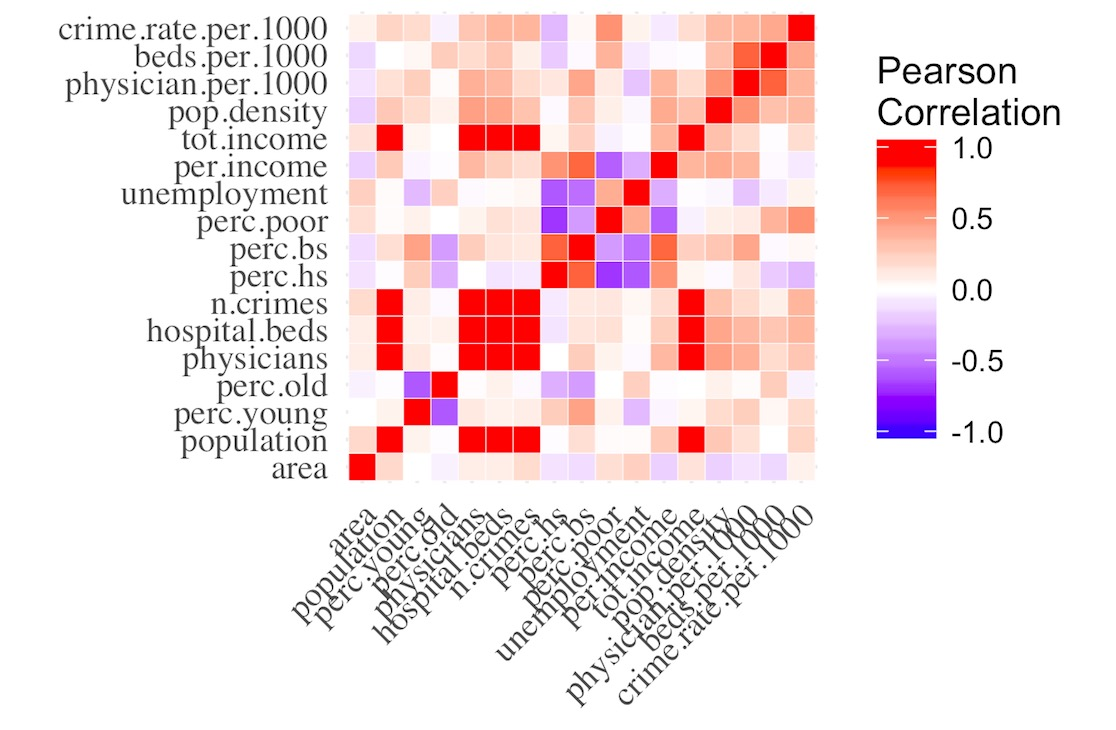
\includegraphics[width=\textwidth]{pics/1.png}}
\caption{Fig.1}
\end{center}


The remaining variables are: area, percentage of young people, percentage of old people, percentage of population with high school degree, percentage of population with bachelor’s degree, poverty rate, unemployment, total income, region, population density, physician per 1000 people, beds per 1000 people.
\begin{center}
  \makebox[\linewidth]{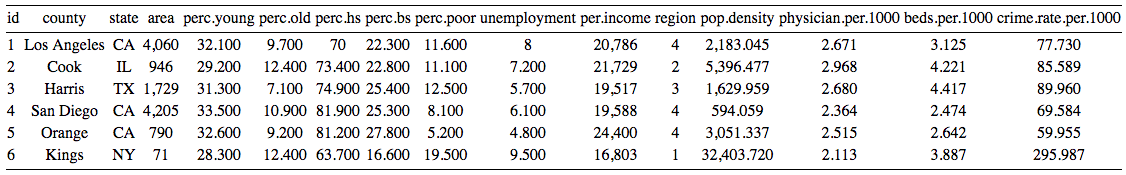
\includegraphics[width=\textwidth]{pics/table1.png}}
      \caption{Table 1}
\end{center}

From Table 1 and Table 2 we can see that Kings county stands out by showing highest population density and highest crime rate among all counties. In the next section we use Poisson Regression Model and Gradient Boosting Model to verify whether it is a coincident.
\begin{center}
  \makebox[\linewidth]{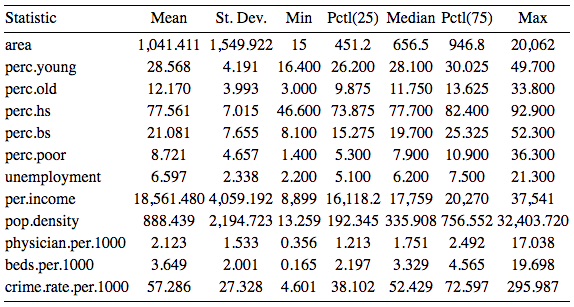
\includegraphics[width=5in]{pics/table2.png}}
    \caption{Table 2}
\end{center}


\section{METHODS}
\label{sec2}
\begin{center}
  \makebox[\linewidth]{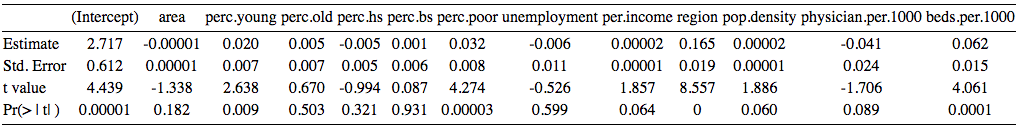
\includegraphics[width=\textwidth]{pics/table3.png}}
      \caption{Table 3}
\end{center}

\indent
We split the data set into training set and test set, then use R to carry out two models, compare their results and use their suggested predictors as complementary to each other.
In the first model we assume that the number of serious crimes in per 1000 people follows a Poisson distribution with mean parameter as linear combination of selected predictors, and we use quasi-likelihood to deal with over-dispersion. After filtering insignificant predictors, our model is as follows:

\begin{align}
log(crime.rate.per.1000) &= \beta_{0} + \beta_{1}\times perc.young + \beta_{2}\times perc.poor\nonumber\\
                         & +\beta_{3}\times per.income + \beta_{42}\times region2 + \beta_{43}\times region3 \nonumber\\
  &+ \beta_{44}\times region4 +\beta_{5}\times log(pop.density) \nonumber\\
  &+ \beta_{6}\times physician.per.1000 + \beta_{7}\times beds.per.1000 \nonumber\\
  &+ \beta_{8}\times perc.bs + \beta_{9}\times unemployment\nonumber
\end{align}


The result is shown in Table 4.
In the second model, we use the same predictors as in first one, but fit a Gradient Boosting Tree Model to the data.
These two models give us consistent results, but slightly different in ranking relative importance of predictors. In the conclusion section we will consider both of them to give our suggestions.



\section{RESULTS}
\label{sec3}

From the result of Poisson Regression Model Table 4, we see that percentage of youth, poverty rate, region, population density and beds per 1000 people are most significant predictors to crime rate. This model suggests that, to obtain 1 unit decrease in crime rate per 1000 people, we should consider (separately) decreasing percentage of youth by exp(0.003) = 1.003, or decreasing poverty rate by exp(0.00003) = 1.00003, or decreasing population density by 0.00003.
Although region plays a significant role here, since it’s impossible to change the region of a county, we can only change other variables that are implicitly related to region.

\begin{center}
  \makebox[\linewidth]{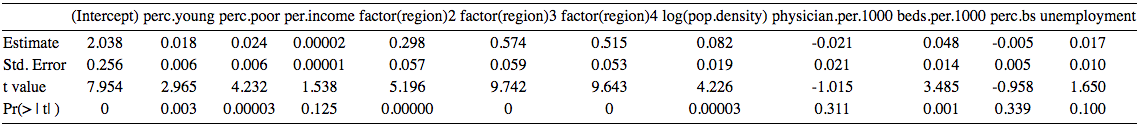
\includegraphics[width=\textwidth]{pics/table4.png}}
      \caption{Table 4}
\end{center}

From the result of Gradient Boosting Model Table 5, we see that most important predictors suggested by this model are: poverty rate, region, physicians per 1000 people, and population density.
\begin{center}
  \makebox[\linewidth]{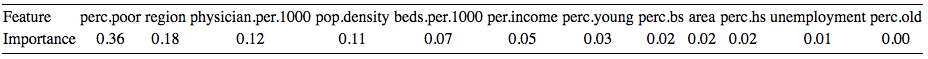
\includegraphics[width=\textwidth]{pics/table5.png}}
      \caption{Table 5}
\end{center}


\begin{figure}[!htb]\centering
   \begin{minipage}{0.49\textwidth}
     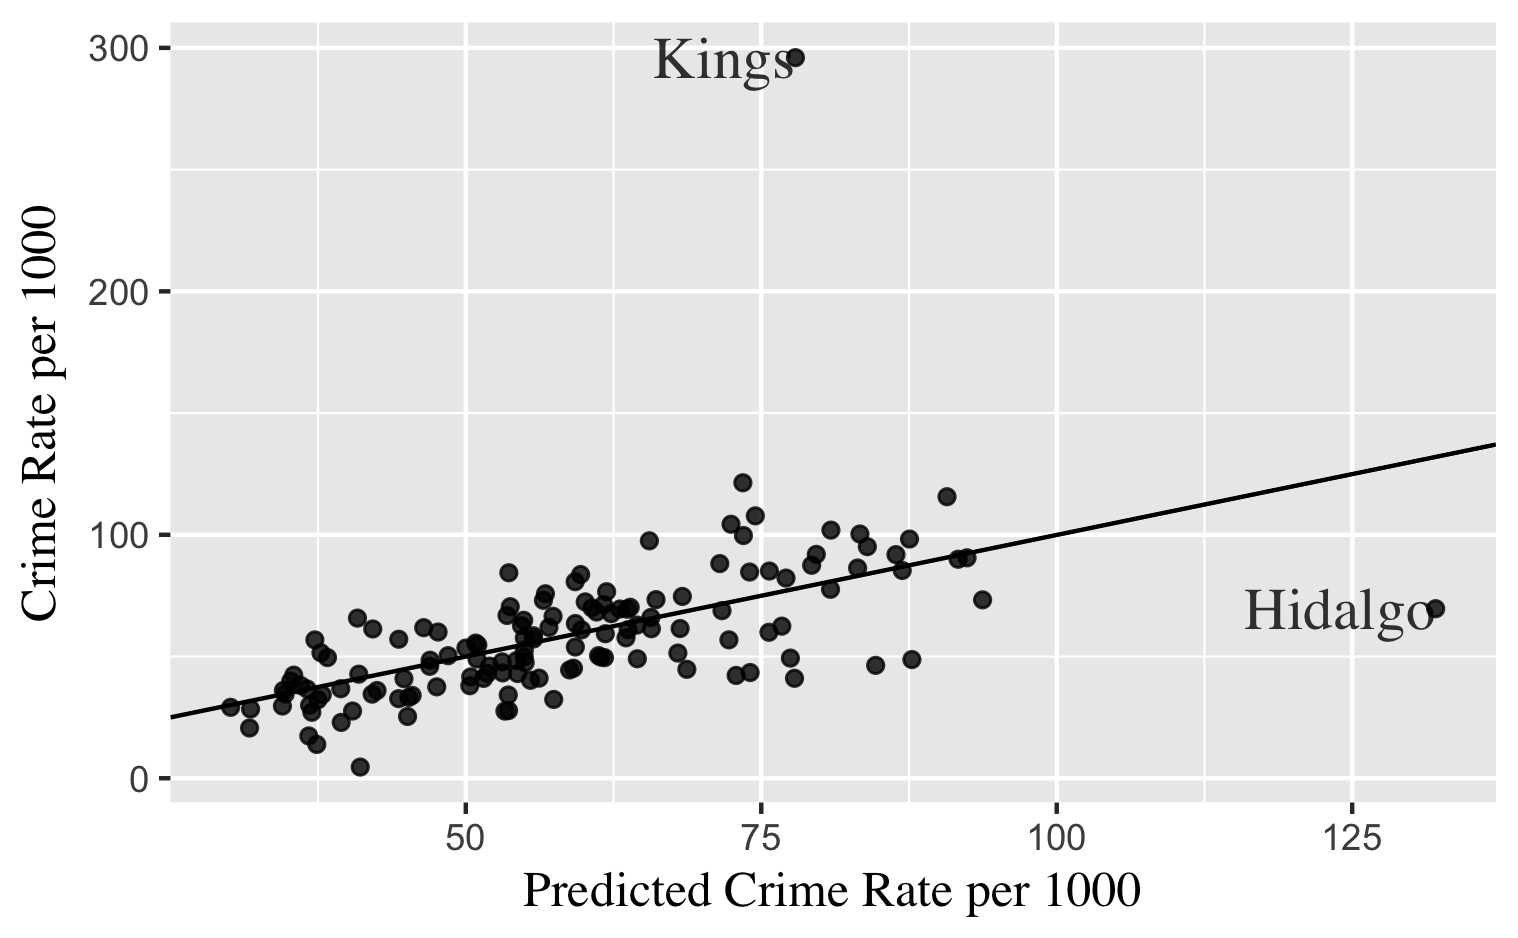
\includegraphics[width=\linewidth]{pics/2.png}
     \label{Fig:Data1}
   \end{minipage}
   \begin {minipage}{0.49\textwidth}
     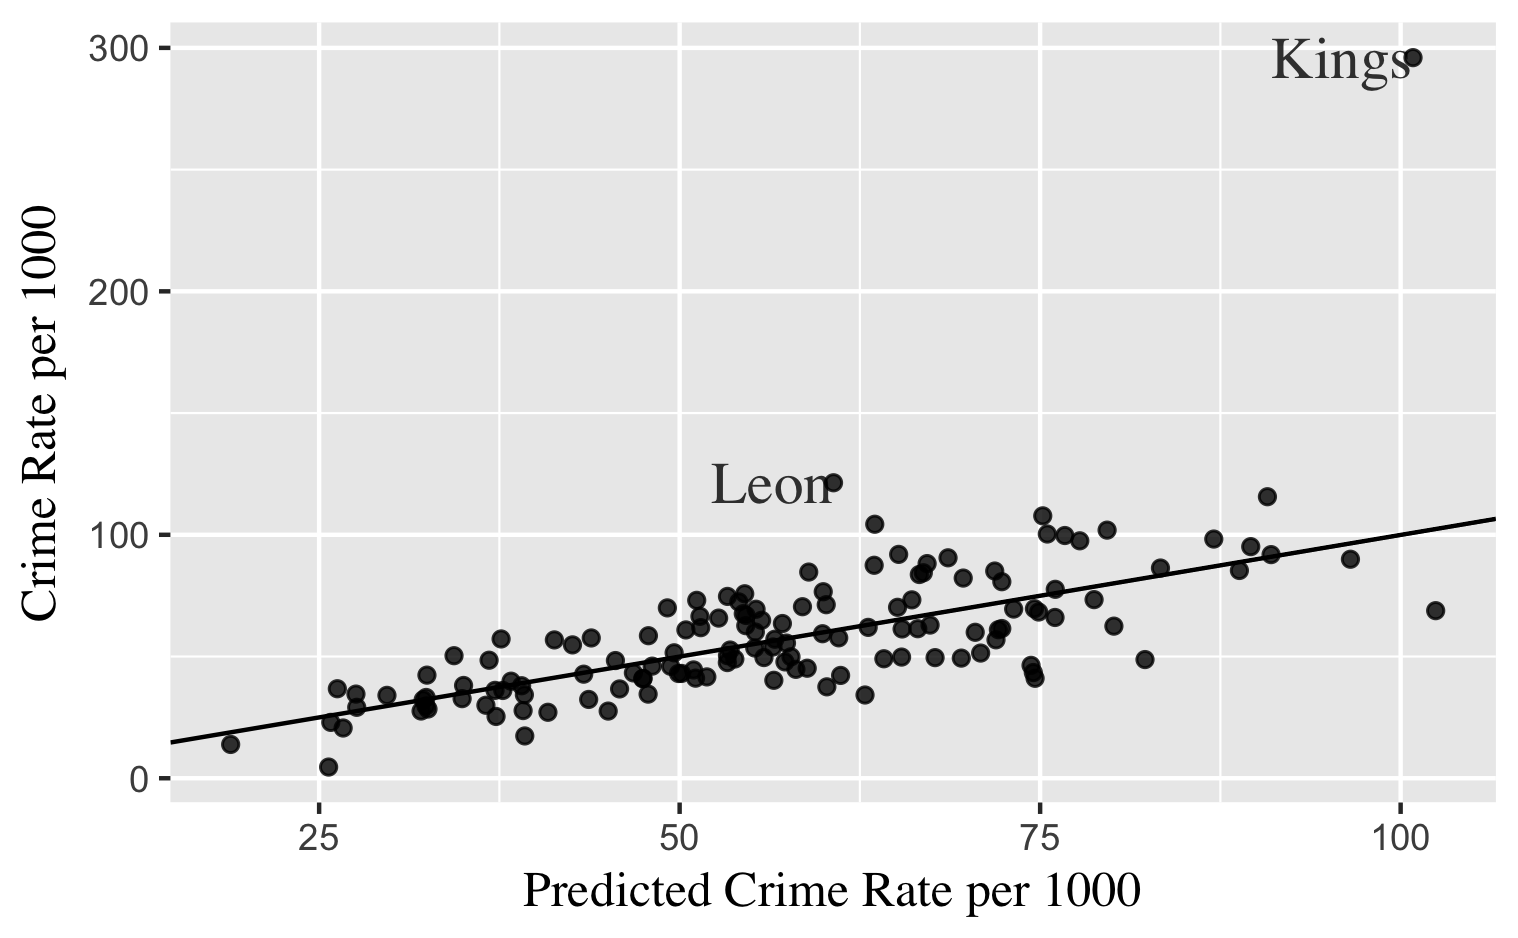
\includegraphics[width=\linewidth]{pics/3.png}
     \label{Fig:Data2}
   \end{minipage}
\end{figure}



Both models are successful in predicting/explaining crime rate in test data, but they fail at one county, our client Kings county.

\begin{center}
  \makebox[\linewidth]{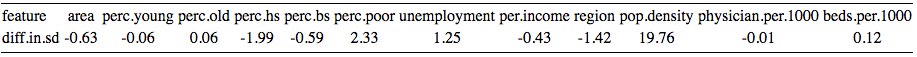
\includegraphics[width=\textwidth]{pics/table6.png}}
      \caption{Table 6}
\end{center}

From Table 6 we see that, in Kings county, poverty rate is of 2.33 standard deviation higher than the average poverty rate in all US counties, and population density is of 19.76 standard deviation higher than the average population density in all US counties.

Since Kings county is located at New York, we also compare Kings county with other counties in New York, and from Table 7 we see that the percentage of population with high school degree in Kings county is of 3.10 standard deviation lower than the average percentage of population with high school degree in all other New York counties, the poverty rate in Kings county is 3.22 standard deviation higher than average other New York counties, and the population density in Kings county is 4.32 standard deviation higher than average other New York counties.

\begin{center}
  \makebox[\linewidth]{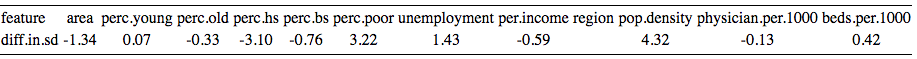
\includegraphics[width=\textwidth]{pics/table7.png}}
      \caption{Table 7}
\end{center}


Now we can give a possible explanation for the failure of our model at Kings county. We suspect that when population density is higher than a threshold, its effect on crime rate would become different from when the population density is lower than that threshold. In other words, as long as population density is not “too high”, the effect of population density on crime rate is restricted, however, once the population density breaks that red line, the crime rate would increase very quickly. Since Kings county is the only county with such high population density (population.png), the parameters obtained from training a model on other counties are actually invalid to it.


\begin{center}
  \makebox[\linewidth]{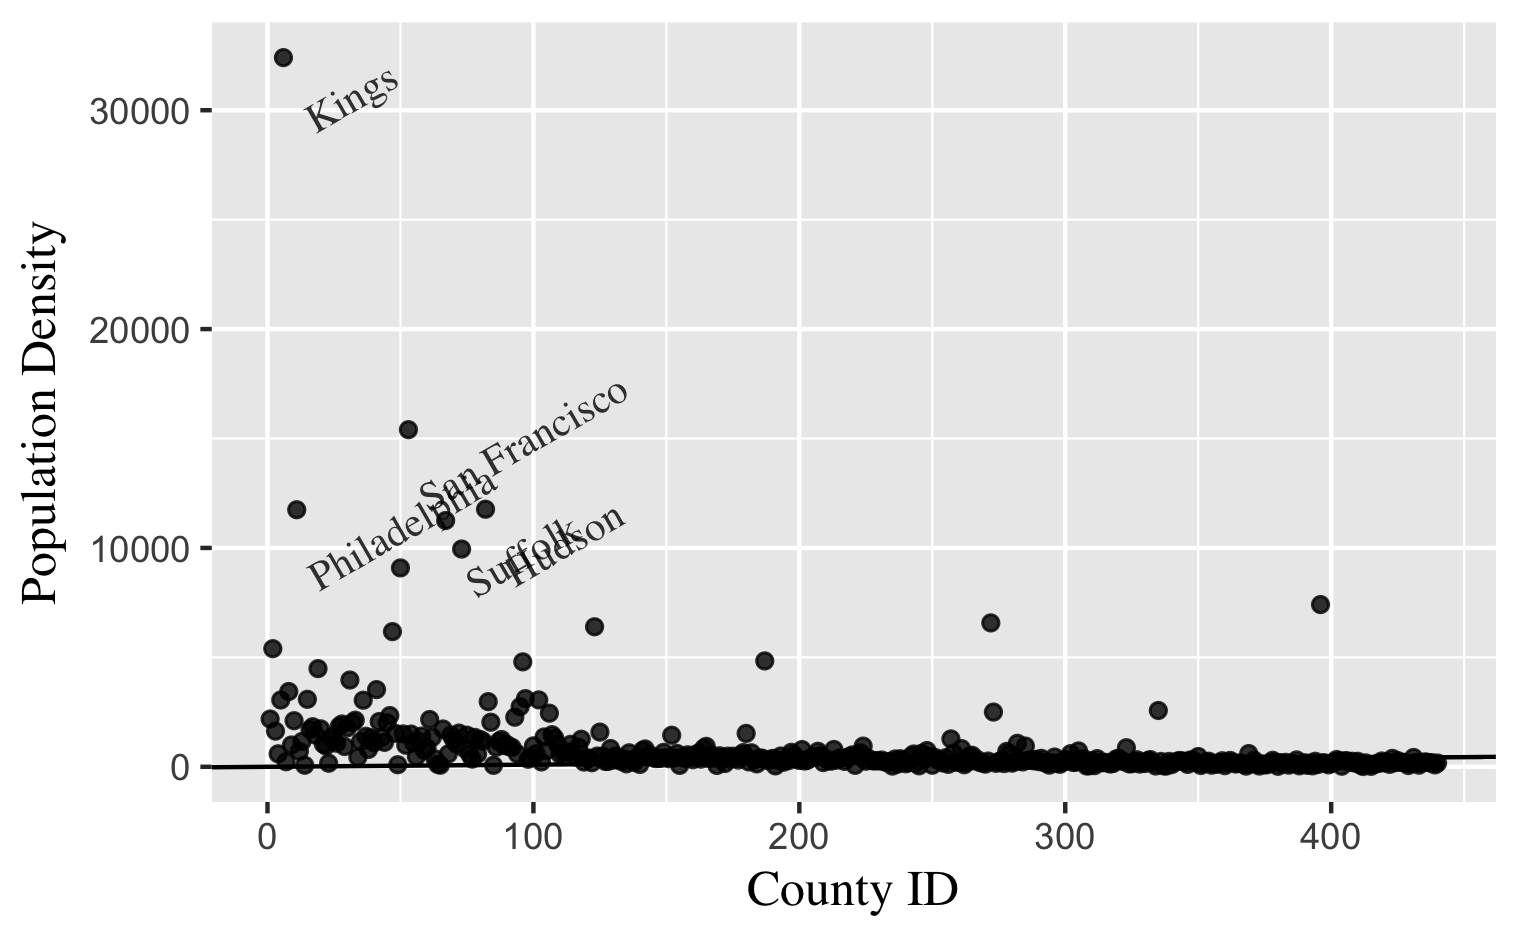
\includegraphics[width=\textwidth]{pics/4.png}}
  \caption{Fig. 4}
\end{center}


\section{CONCLUSION}
\label{sec4}
Given above analysis, we provide slightly different suggestions to Kings county and to potential clients who are suffering from high crime rate.
\bigbreak
\textbf{General suggestions}:
\begin{itemize}
  \setlength\itemsep{0em}
  \item Reduce poverty rate by providing food, shelter and career training to low-income people.
  \item Educate young people about how to resolve disputes and conflicts through law process.
\item Equip hospitals with more physicians and beds.
\end{itemize}
\bigbreak
%\noindent
\textbf{Specific suggestion for Kings county}:
\begin{itemize}
\item Increase effective land area, provide assistance to people who are willing to relocate.
\end{itemize}


\section{REFERENCE}
\label{sec5}


\begin{thebibliography}{25}
\bibitem{latexcompanion}
What Statistical Consultants Do: Report of a Survey\\
\texttt{http://csyue.nccu.edu.tw/ch/What Statistical Consultants Do Report of a Survey.pdf}

\bibitem{latexcompanion}
Interpreting Crime Data and Statistics\\
\texttt{http://www.iaca.net/ExploringCA/2Ed/exploringca\_chapter8.pdf}

\bibitem{latexcompanion}
A Stargazer Cheatsheet\\
\texttt{http://jakeruss.com/cheatsheets/stargazer.html}

\end{thebibliography}
% https://www.sharelatex.com/learn/Bibliography_management_with_bibtex



%% The Appendices part is started with the command \appendix;
%% appendix sections are then done as normal sections



%% References
%%
%% Following citation commands can be used in the body text:
%% Usage of \cite is as follows:
%%   \cite{key}         ==>>  [#]
%%   \cite[chap. 2]{key} ==>> [#, chap. 2]
%%

%% References with bibTeX database:

\bibliographystyle{elsarticle-num}
% \bibliographystyle{elsarticle-harv}
% \bibliographystyle{elsarticle-num-names}
% \bibliographystyle{model1a-num-names}
% \bibliographystyle{model1b-num-names}
% \bibliographystyle{model1c-num-names}
% \bibliographystyle{model1-num-names}
% \bibliographystyle{model2-names}
% \bibliographystyle{model3a-num-names}
% \bibliographystyle{model3-num-names}
% \bibliographystyle{model4-names}
% \bibliographystyle{model5-names}
% \bibliographystyle{model6-num-names}

\bibliography{sample}


\end{document}

%%
%% End of file `elsarticle-template-num.tex'.
